\section{Eliminacja lewostronnej rekurencji}
ANTLR wspiera bezpośrednie lewostronnie rekurencyjne reguły przez przepisanie ich
na nie-lewostronnie rekurencyjną wersję która również usuwa niejednoznaczność.
Na przykład, naturalna gramatyka do opisu składni wyrażeń arytmetycznych
jest jedną z najbardziej rozpowszechnionych (niejednoznacznych)
lewostronnie rekurencyjnych reguł. Następująca gramatyka obsługuje proste wyrażenia modulo i dodawanie.
\par
$E \rightarrow E\%E | E+E | id$
\par
E jest bezpośrednio lewostronnie rekurencyjna ponieważ co najmniej jedna produkcja zaczyna się od 
E ($\exists E \Rightarrow E\alpha$), co jest problemem dla zstępujących parserów.
\par
Gramatyki znaczące dla zstępujących parserów muszą użyć kłopotliwego 
nie lewostronnie rekurencyjnego odpowiednika mającego oddzielny
nieterminal dla każdego poziomu priorytetu operatora:
\begin{itemize}
\item $E' \rightarrow M (+ M)^*$ Dodawanie, niski priorytet
\item $M \rightarrow P (\% P)^*$ Modulo, wyższy priorytet
\item $P \rightarrow id$ Primary (id oznacza identyfikator)
\end{itemize}
Im głębsze jest wywołanie reguły, tym wyższy priorytet.
Podczas czasu parsowania dopasowanie pojedynczego identyfikatora
wymaga wywołania jednej reguły dla jednego poziomów priorytetu.
\par
E jest łatwiejsze do czytania niż E', ale lewostronnie rekurencyjna wersja jest
niejednoznaczna ponieważ są dwie interpretacje wejścia a+b+c:
(a+b)+c i a+(b+c). Generatory parserów wstępujących takie jak bison 
używają specyfikatorów priorytetu operatorów (e.g., \%left '\%') do
rozwiązania takiej niejednoznaczności.
Nie lewostronnie rekurencyjna gramatyka E'
jest jednoznaczna ponieważ niejawnie koduje reguły priorytetu
według głębokości zagnieżdżenia nieterminalu.
\par
Idealnie, parser powinien wspomagać lewostronną rekurencję i
dostarczać sposobu do rozwiązania niejednoznaczności niejawnie 
przez samą gramatykę bez uciekania się do zewnętrznych specyfikatorów priorytetu.
ANTLR robi to przez przepisanie nieterminali z bezpośrednią lewostronną rekurencją 
i wstawienie semantycznych predykatów by rozwiązać niejednoznaczność
zgodnie z porządkiem produkcji. Proces przepisywania
prowadzi do generowanych parserów które imitują technikę Clarke'a [5].
\par
Wybraliśmy do eliminacji tylko bezpośrednią lewostronną rekurencję ponieważ ogólna eliminacja lewostronnej 
rekurencji może skutkować transformowanymi gramatykami o rząd wielkości większymi niż oryginalna [11] i
dostarczać drzewa parsowania jedynie luźno powiązane do tych z oryginalnej gramatyki.
ANTLR automatycznie konstruuje drzewa parsowania zgodne z oryginalną lewostronnie rekurencyjną 
gramatyką
tak że programista jest nie powiadomiony o wewnętrznej restrukturyzacji.
Lewostronna rekurencja również pokrywa większość powszechnych gramatycznych przypadków (z długiego
doświadczenia budowania gramatyk). Ta dyskusja skupia się na gramatykach dla wyrażeń arytmetycznych ale 
reguły transformacji działają równie dobrze dla innych lewostronnie rekurencyjnych konstrukcji takich jak 
deklaracje C:
$D\rightarrow *D$,$D\rightarrow D[]$,$D\rightarrow D()$,$D\rightarrow id$
\par
Eliminacja bezpośredniej lewostronnej rekurencji bez koncentrowania się na niejednoznaczności jest prosta
 [11]. Niech $A \rightarrow \alpha_j$ dla j = 1..s będzie nie lewostronnie rekurencyjnymi
produkcjami $A \rightarrow A \beta_k$ dla k = 1..r będzie bezpośrednimi lewostronnymi
produkcjami gdzie $\alpha_j$,$\beta_k$ $\nRightarrow^* \epsilon$.
Zastąpimy te produkcje przez:
\begin{itemize}
\item $A \rightarrow \alpha_1 A'|..|\alpha_s A'$
\item $A'\rightarrow \beta_1A'|...|\beta_rA'|\epsilon$
\end{itemize}
Łatwiej jest zobaczyć transformację używając EBNF:
\begin{itemize}
\item $A \rightarrow A' A'' *$
\item $A' \rightarrow \alpha_1|...|\alpha_s$
\item $A'' \rightarrow \beta_1|...|\beta_r$
\end{itemize}
albo właśnie $A \rightarrow (\alpha_1|...|\alpha_s)(\beta_1|...|\beta_r)*$
Na przykład lewostronnie rekurencyjna reguła E staje się:
\par
$E \rightarrow id (\%E|+E)^*$
\par
Ta nie lewostronnie rekurencyjna wersja pozostaje niejednoznaczna ponieważ są dwa wyprowadzenia dla 
a+b+c. Domyślnie polityka rozwiązywania niejednoznaczności wybiera do dopasowania tak dużo symboli 
wejściowych jak to jest możliwe dając interpretację (a+b)+c.
\par
Różnica w łączności nie ma znaczenia w wyrażeniach używających pojedynczego operatora ale wyrażenia z 
mieszaniną operatorów muszą łączyć operandy i operatory zgodnie z priorytetem operatorów, Na przykład, 
parser musi rozpoznawać a\%b+c jako (a\%b)+c a nie a\%(b+c).
Dwie interpretacje są pokazane na Rysunku 14.

\begin{figure}[h]
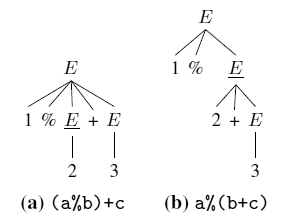
\includegraphics[scale=0.67]{Figure14.png}
\caption{Drzewa parsowania dla a\%b+c i $E\rightarrow(\%E|+E)^* $}
%i $$}
\end{figure}

Aby wybrać właściwą interpretację , generowany parser
musi porównać priorytet poprzedniego operatora do priorytetu bieżącego operatora
w $(\% E | + E)^*$ w "pętli." Na Rysunku 14, underscore{E} jest krytyczna ekspansją E.
Musi jedynie dopasować id i od
razu powrócić, pozwalając wołanemu E dopasować + do formy drzewa parsowania (a) lub odwrotnie (b).
\par
Aby obsługiwać takie porównania, produkcje dostają numer priorytetu, który jest przeciwieństwem numeru 
produkcji. Priorytet i-tej produkcji jest n-i+1 dla n \textit{oryginalnych} produkcji E.
To przypisuje priorytet 3 do $E \rightarrow E \%E$, priorytet 2 do
$E \rightarrow E + E$ i priortyet 1 do $E \rightarrow id$.
\par
Następnie każde zagnieżdżone wywołanie E potrzebuje informacji 
o priorytecie operatora z wołanego E. Najprostszym mechanizmem
jest włożenie parametru priorytetu pr do E:
\textit{Rozwinięcie E[pr] może dopasować jedynie te podwyrażenia
których priorytet odpowiada albo przekracza pr.}
\par
By zmusić do tego, procedura eliminacji lewostronnej rekurencji 
wstawia predykaty do pętli (\% E | + E)*. Tutaj jest transformowana
jednoznaczna i nie lewostronnie rekurencyjna reguła:
\par
$E[pr] \rightarrow \textbf{id} (\{ 3 \geq pr\}? \%E[4]| \{ 2 \geq pr\}?+E[3])^*$
\par
Odniesienia do E wszędzie w gramatyce stają się E[0]: czyli $S\rightarrow E$ staje się $S\rightarrow E[0]$.
Wejście a\%b+c daje drzewo parsowania dla E[0] pokazane na (a) obrazka 15.
\begin{figure}[h]
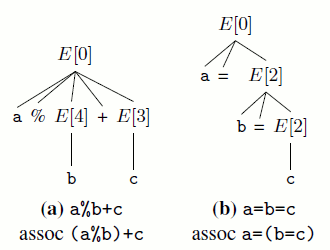
\includegraphics[scale=0.67]{Figure15.png}
\caption{Drzewa Rozwinięcia Nieterminali dla nieterminalu
$E[pr]\rightarrow id (\{3 \geq pr \}? \%E[4]|\{2 \geq pr \}? +E[3])^* $}
%i $$}
\end{figure}
\par
Produkcja “$\{ 3 \geq pr\}? \%E[4]$” jest wykonalna kiedy priorytet
operacji modulo 3, odpowiada lub przekracza parametr pr.
Pierwsze wołanie E ma pr = 0 i ponieważ $3 \geq 0$
parser rozwija “\% E[4]” w E[0].
\par
Kiedy wołamy parsowanie E[4], predykat $ {2 \geq pr}?$ nie przechodzi
ponieważ priorytet operatora + jest zbyt niski: $2 \ngeq 4$.
Konsekwentnie E[4] nie dopasowuje operatora + opóźniając
wołanie E[0].
\par
Kluczowym elementem transformacji jest wybór 
parametrów E, E[4] i E[3] w tej gramatyce. Dla operatorów lewostronnej łączności
jak \% i +, prawy operand dostaje o jeden stopień priorytetu więcej niż sam operator.
To gwarantuje że wołanie E dla prawego operandu dopasuje wyłącznie operacje wyższego priorytetu.
\par
Dla prawostronnie łącznych operacji. operand E dostaje ten sam priorytet
co bieżący operator. Tutaj jest wariacja gramatyki wyrażenia która ma prawostronny 
operator przypisania zamiast operatora dodawania:
\par
$E \rightarrow E \% E |E =^right E | \textbf{id}$
\par
gdzie notacja =^right jest skrótem dla rzeczywistej ANTLR
składni “|<assoc=right> E =^right E.” 
Interpretacja a=b=c powinna być prawostronnie łącznam a=(b=c). Aby dostać łączność,
transformowana reguła potrzebuje różnić się wyłącznie w prawym 
operandzie, E[2] kontra E[3]:
\par
$E[pr] \rightarrow \textbf{id} (\{3 \geq pr\}? \%E[4] |\{2\geq pr\}? = E[2])*$
\par
Rozwinięcie E[2] może dopasować przypisanie jak pokazano na (b) Obrazka 15, ponieważ predykat
$2 \geq 2$ jest true.
\par
Operatory unarnych prefiksów i sufiksów są natomiast traktowane jako prawe lewostronnie łączne.
Rozważmy następujące E z prefiksem negacji i sufiksem „not”.
\par
$E \rightarrow -E |E !|E \%E | \textbf{id}$
\par
Operatory prefiksu nie są lewostronnie rekurencyjne i stąd idą do
pierwszej podreguły podczas gdy lewostronnie rekurencyjne operaotry sufiksu idą do pętli predykatu 
jak operatory binarne:
\par
$E[pr] \rightarrow (id | - E[4])$
$(\{3 |wieksze_rowne pr\}? !| \{2 \geq pr\}? \%E[3])*$
\begin{figure}[h]
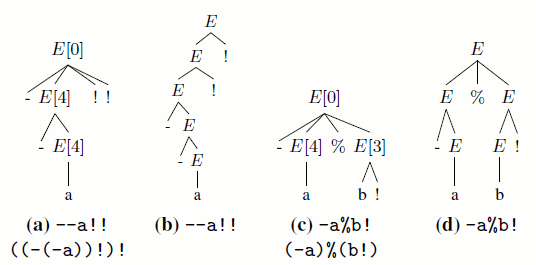
\includegraphics[scale=0.67]{Figure16.png}
\caption{Drzewa wołania nieterminali i drzewa parsowania dla prdukcji
$E\rightarrow-E|E!|E\%E|id$}
%i $$}
\end{figure}
Obrazek 16 ilustruje drzewo wołania reguł (zapis stosu wowołań) i powiązane drzewa parsowania będące
rezultatem parsera generowanego przez ANTLR. Operacje unarne w przyległych produkcjach wszystkie mają
ten sam relatywny priorytet i są dlatego “wyliczane” w podanej kolejności.
Czyli
$E \rightarrow -E | + E | id$ musi interperatować -+a jako -(+a) nie +(-a).
\par
Nonkonformistyczne leowstronne produkcje $E \rightarrow E$ lub
$E \rightarrow \epsilon $ są przepisane bez koncentrowania się na niejednoznaczności używając typowych
technik eliminacji.
\par
Ponieważ potrzeba rozwiązania niejednoznaczności z predykatami i obliczenia parametrów A
